\begin{figure*}[htbp]
    \centering
    \begin{subfigure}[b]{0.49\textwidth}
       \centering
       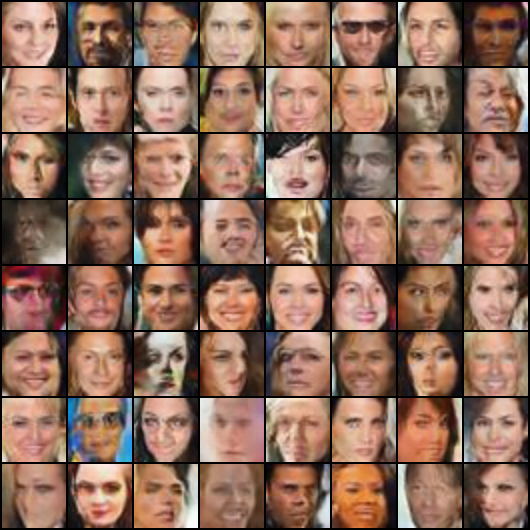
\includegraphics[width=\exfactor\textwidth]{figures/celeba/31_base_raw_base.png}
       \caption{GAN}
    \end{subfigure}
    \begin{subfigure}[b]{0.49\textwidth}
       \centering
       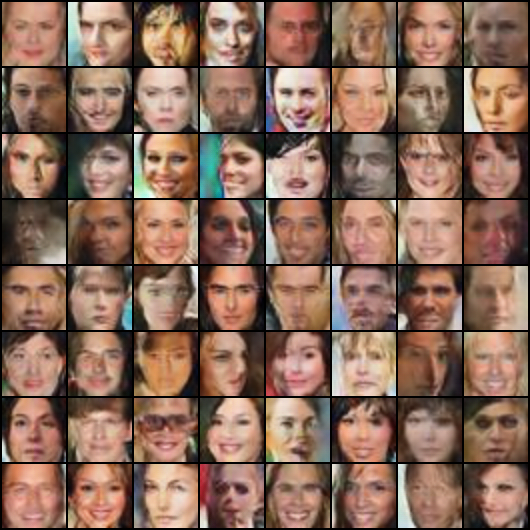
\includegraphics[width=\exfactor\textwidth]{figures/celeba/31_base_raw_reject.png}
       \caption{DRS}
    \end{subfigure}
    \begin{subfigure}[b]{0.49\textwidth}
       \centering
       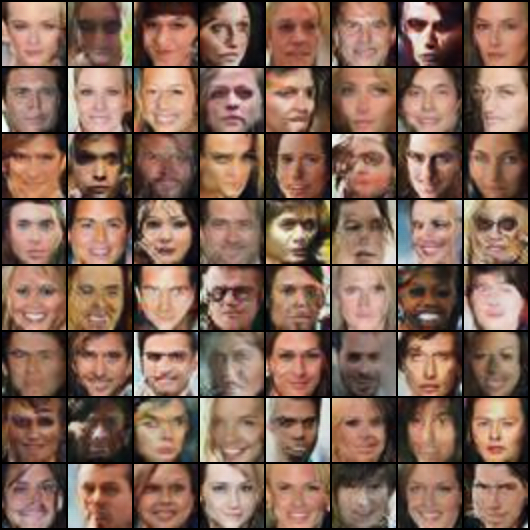
\includegraphics[width=\exfactor\textwidth]{figures/celeba/31_base_raw_MH.png}
       \caption{MH-GAN}
    \end{subfigure}
    \begin{subfigure}[b]{0.49\textwidth}
       \centering
       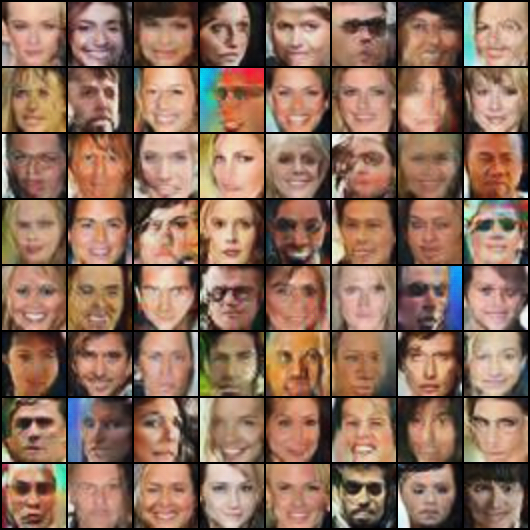
\includegraphics[width=\exfactor\textwidth]{figures/celeba/31_base_iso_MH.png}
       \caption{MH-GAN (cal)}
    \end{subfigure}
    \caption{
    Example images on CelebA for different GAN setups.
    Like Figure~\ref{fig:cifar_samples}, the same batch of images goes into each selector.
    }
    \label{fig:celeba_samples}
\end{figure*}
